\section{Research trends in agent-based modeling}

\subsection{From methodological niche to cross-domain infrastructure}

\begin{figure}[htbp]
\centering
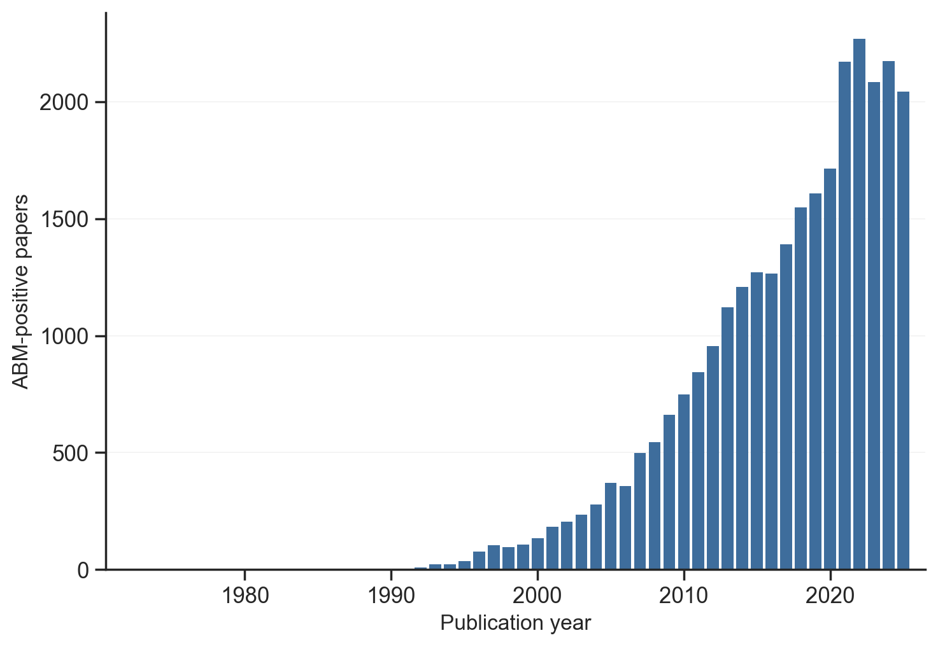
\includegraphics[width=0.96\textwidth,height=0.78\textheight,keepaspectratio]{figures/figure_02.png}
\setcounter{figure}{1}
\caption{Annual publication counts for the strict ABM corpus, 1972–2025 (n = 29,139).}
\label{fig:figure2}
\end{figure}

ABM research expanded steadily and diversified across disciplines. The corpus grew approximately nineteen-fold between 2000 and 2025, marking a shift from a specialized simulation approach to a framework used across many research areas. The increase was not a single abrupt departure from the previous trend. A segmented Poisson model identified 2021 as a potential breakpoint and estimated a 24.0\% increase in publication intensity (z = 6.36, p = 2.0 × 10−10). Yet observed output in 2021–2023 (3,774 papers) was close to the pre-breakpoint projection (3,945 papers), with no significant excess (rate ratio = 0.957, p = 0.997). After adjustment for overall retrieval trends, the estimated change associated with this high-growth period was also not significant (−1.8\%, p = 0.846).

Taken together, the analyses are more consistent with cumulative diffusion across scientific domains than with a single external shock. Publication growth alone, however, cannot show how the field itself changed. The next sections therefore examine domain composition and thematic shifts, separating expansion in the number of papers from redistribution of attention across research areas.

\subsection{Thematic reorientation}

The corpus spans a broad range of applications, although a few domains account for much of the research. Epidemiology and public health is the largest identified domain (7,271 papers; 24.95\%), followed by simulation methodology (4,986; 17.11\%) and ecology and environment (4,564; 15.66\%). The two leading application domains—epidemiology/public health and ecology/environment—together represent 40.62\% of the corpus. Transport (9.79\%), social and opinion dynamics (8.53\%), and urban and land-use systems (6.70\%) form a second tier. This distribution is consistent with ABM’s value for studying interactions among heterogeneous entities and their aggregate consequences. The substantial methodology category also shows that growth includes continued work on ABM itself, not applications alone.

\begin{figure}[htbp]
\centering
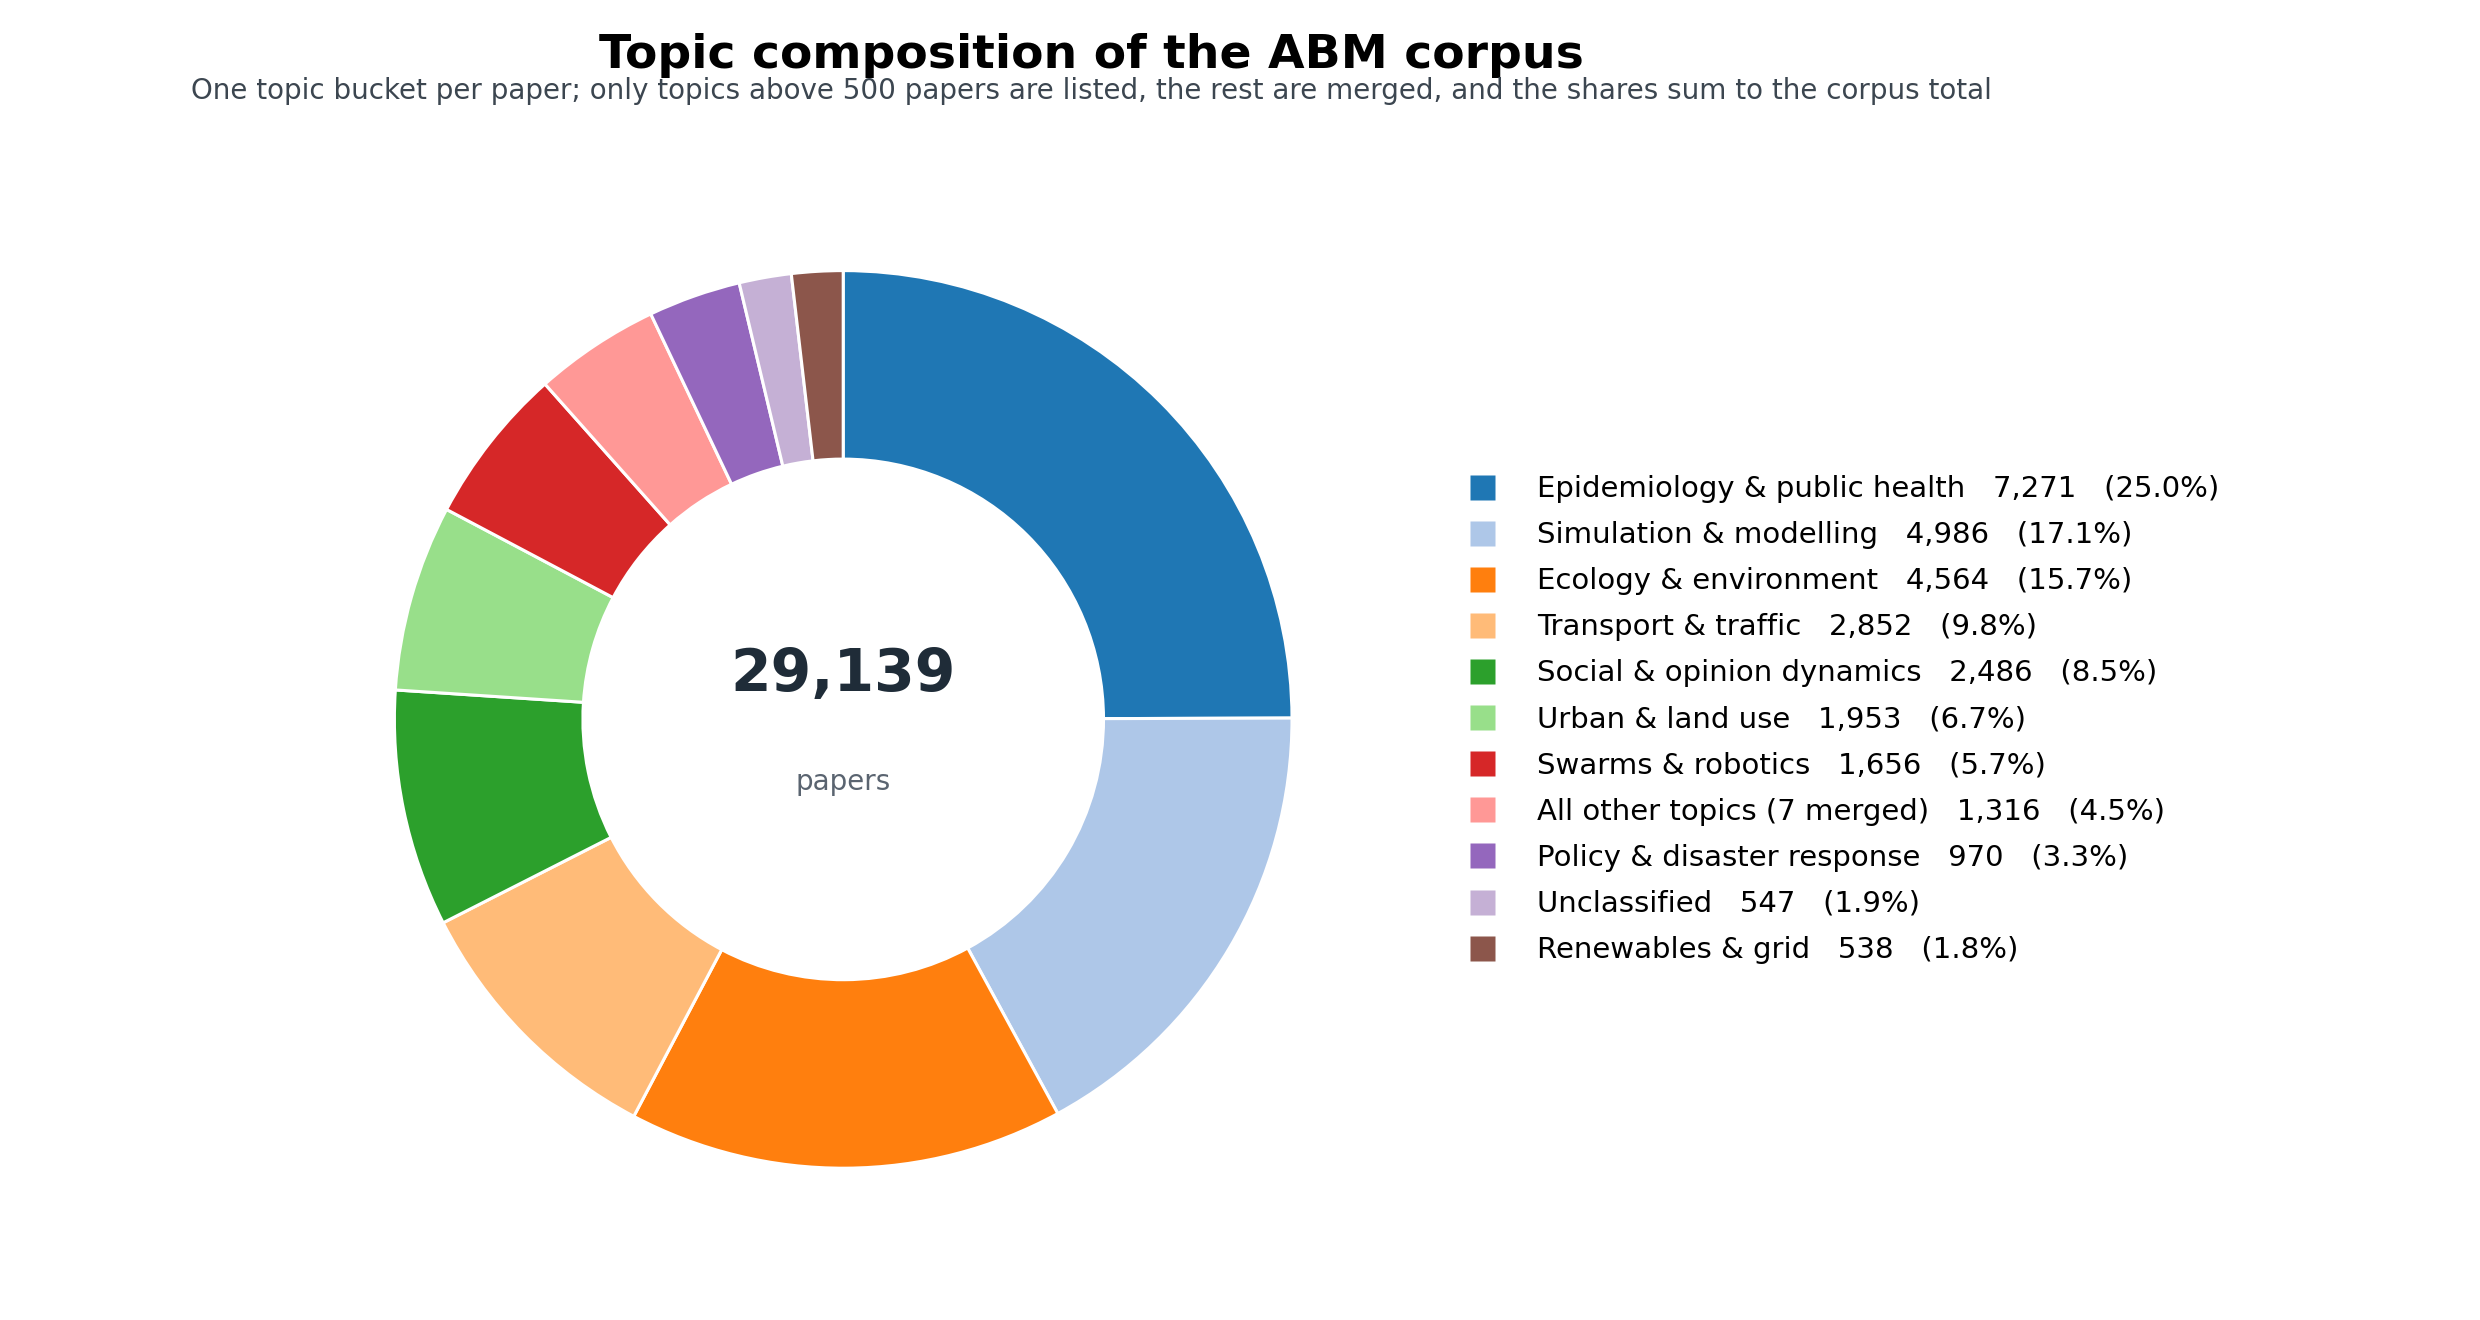
\includegraphics[width=0.96\textwidth,height=0.78\textheight,keepaspectratio]{figures/figure_03.png}
\setcounter{figure}{2}
\caption{Overall thematic composition of the ABM corpus.}
\label{fig:figure3}
\end{figure}

The annual series shows that the field’s composition changed alongside its overall growth. Ecology and environment declined from about 28.0\% of papers in 2001 to roughly 15\% in 2025. Epidemiology and public health rose from about 15.3\% in 2001, peaked at 40.9\% in 2022, and remained the leading application family through 2025. Transport also gained share—from roughly 2–3\% around 2000 to about 11\% in 2025—while social and opinion dynamics became an established line of work. These changes indicate a broader portfolio in which human behavior, institutions, mobility, communication, and policy are studied alongside environmental processes; they do not mean that earlier areas have disappeared.

\begin{figure}[htbp]
\centering
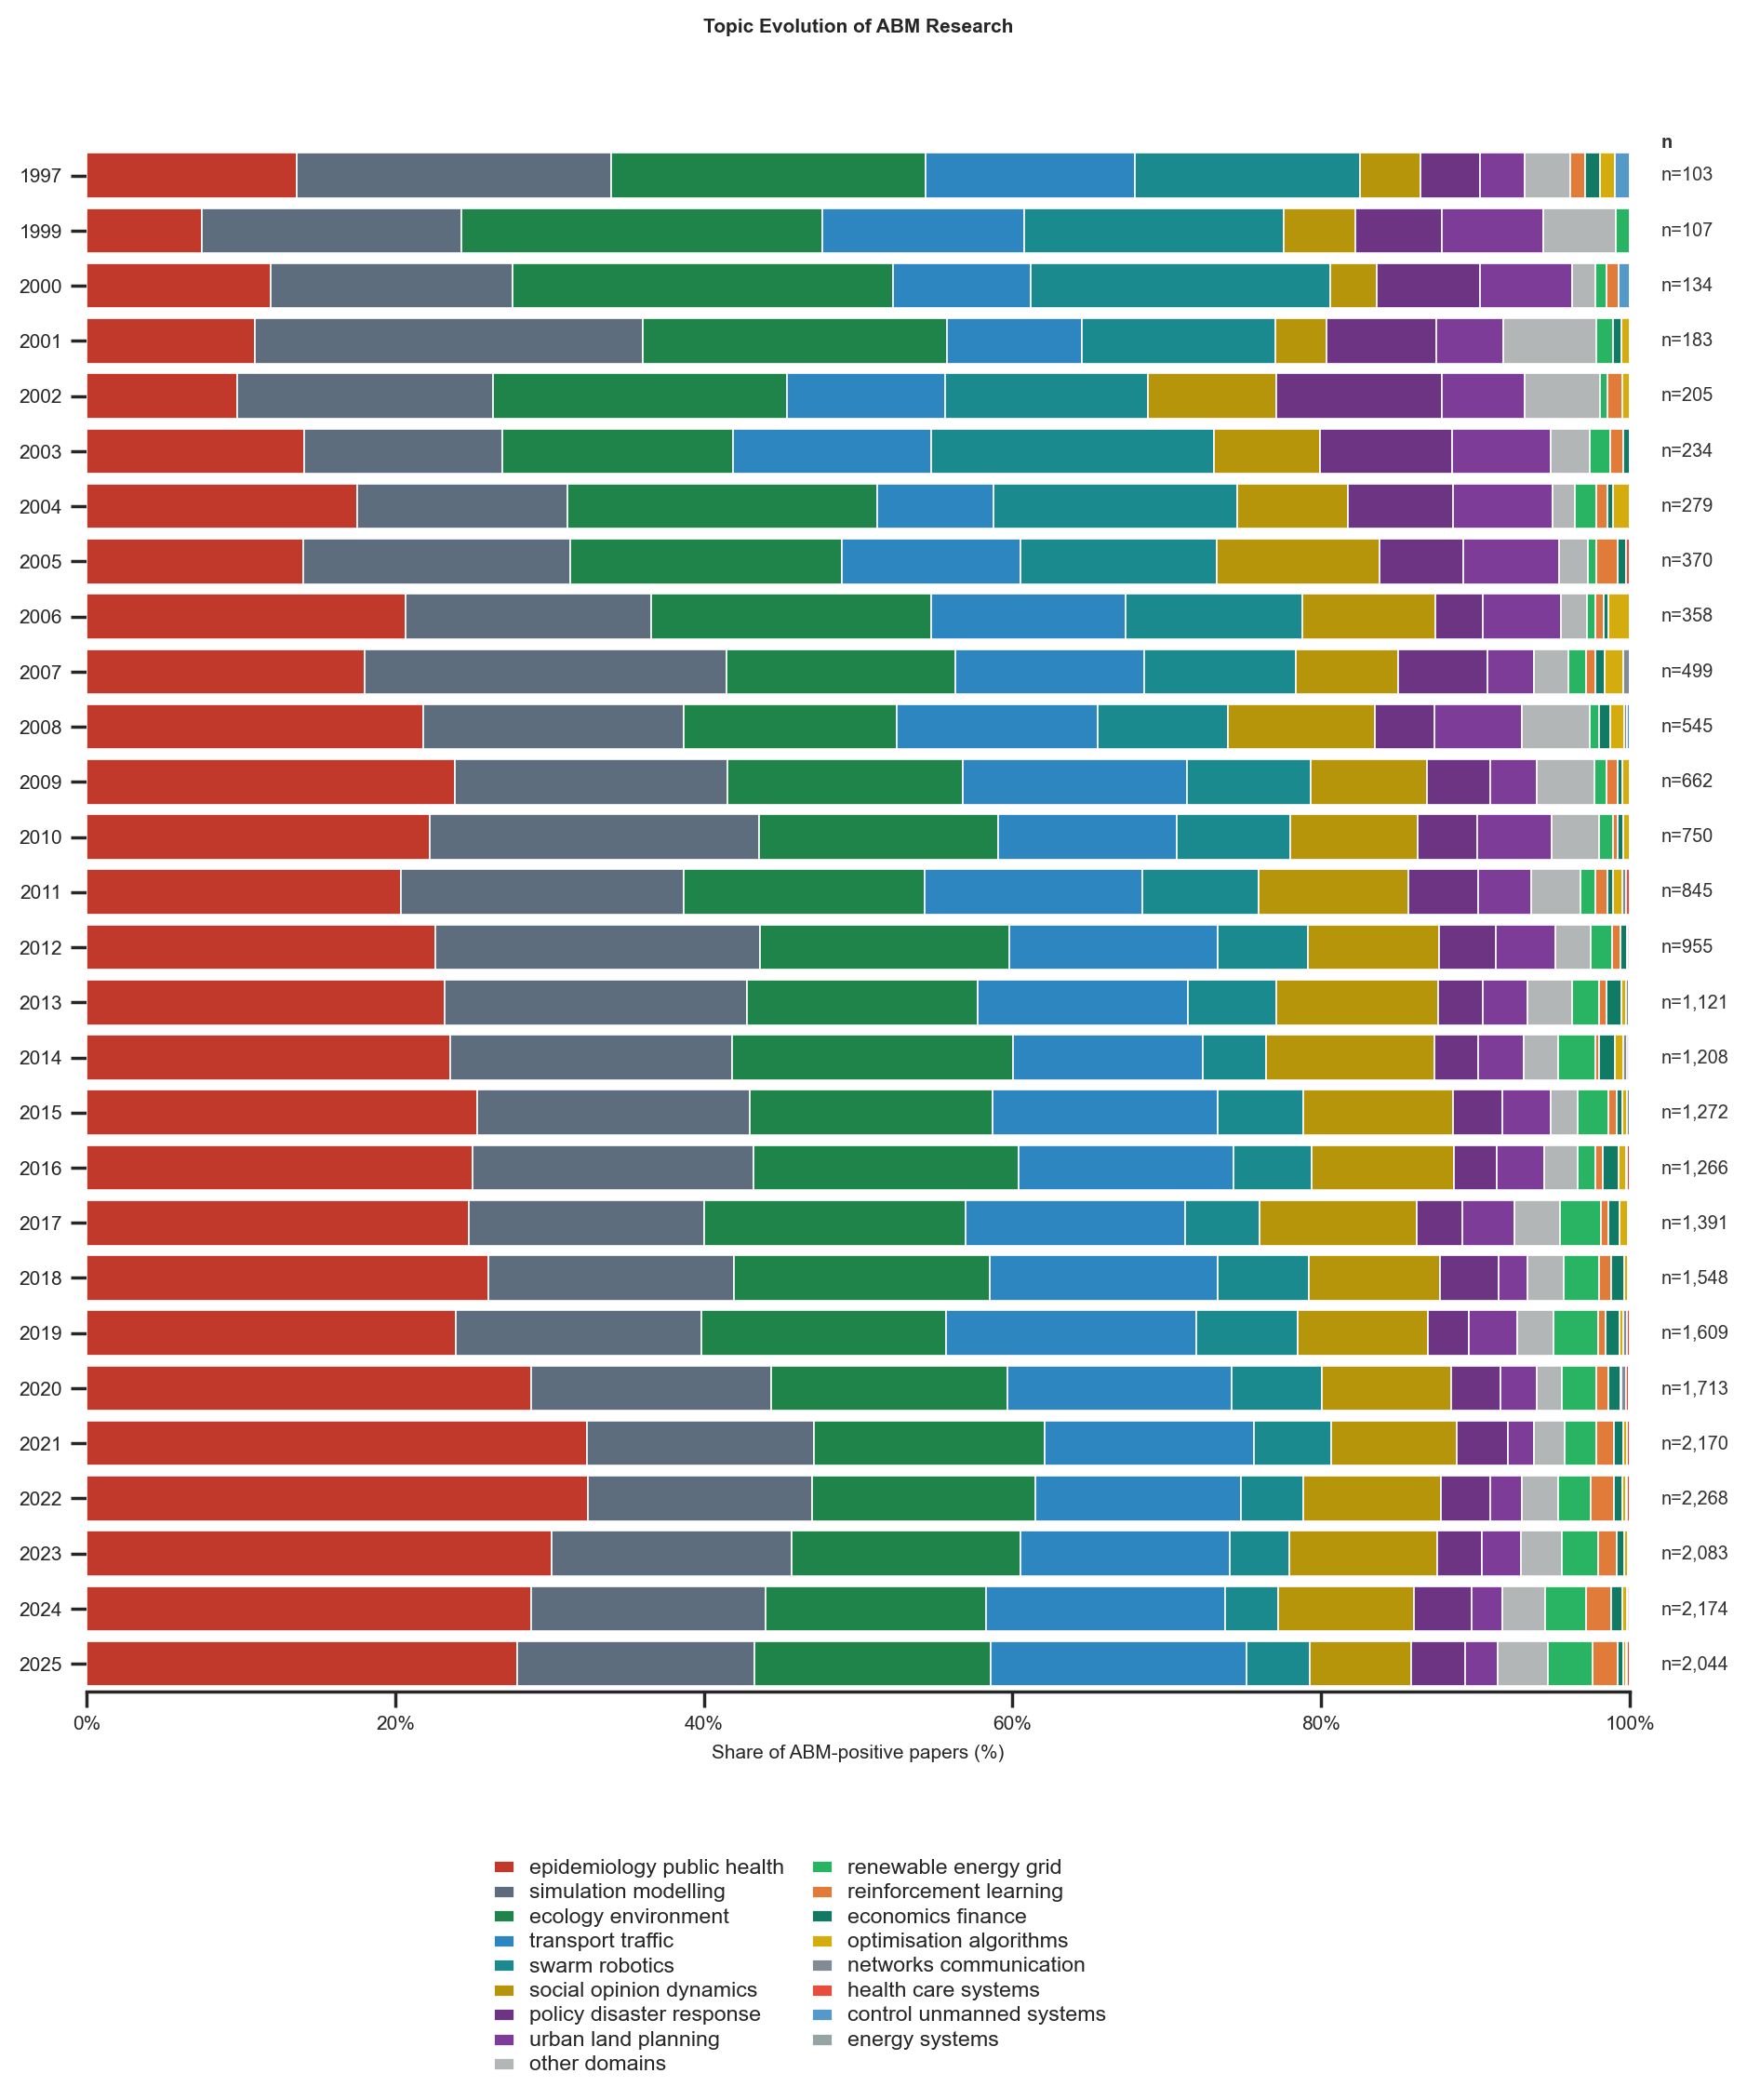
\includegraphics[width=0.96\textwidth,height=0.78\textheight,keepaspectratio]{figures/figure_04.png}
\setcounter{figure}{3}
\caption{Annual evolution of thematic composition, 2001–2025.}
\label{fig:figure4}
\end{figure}

\begin{figure}[htbp]
\centering
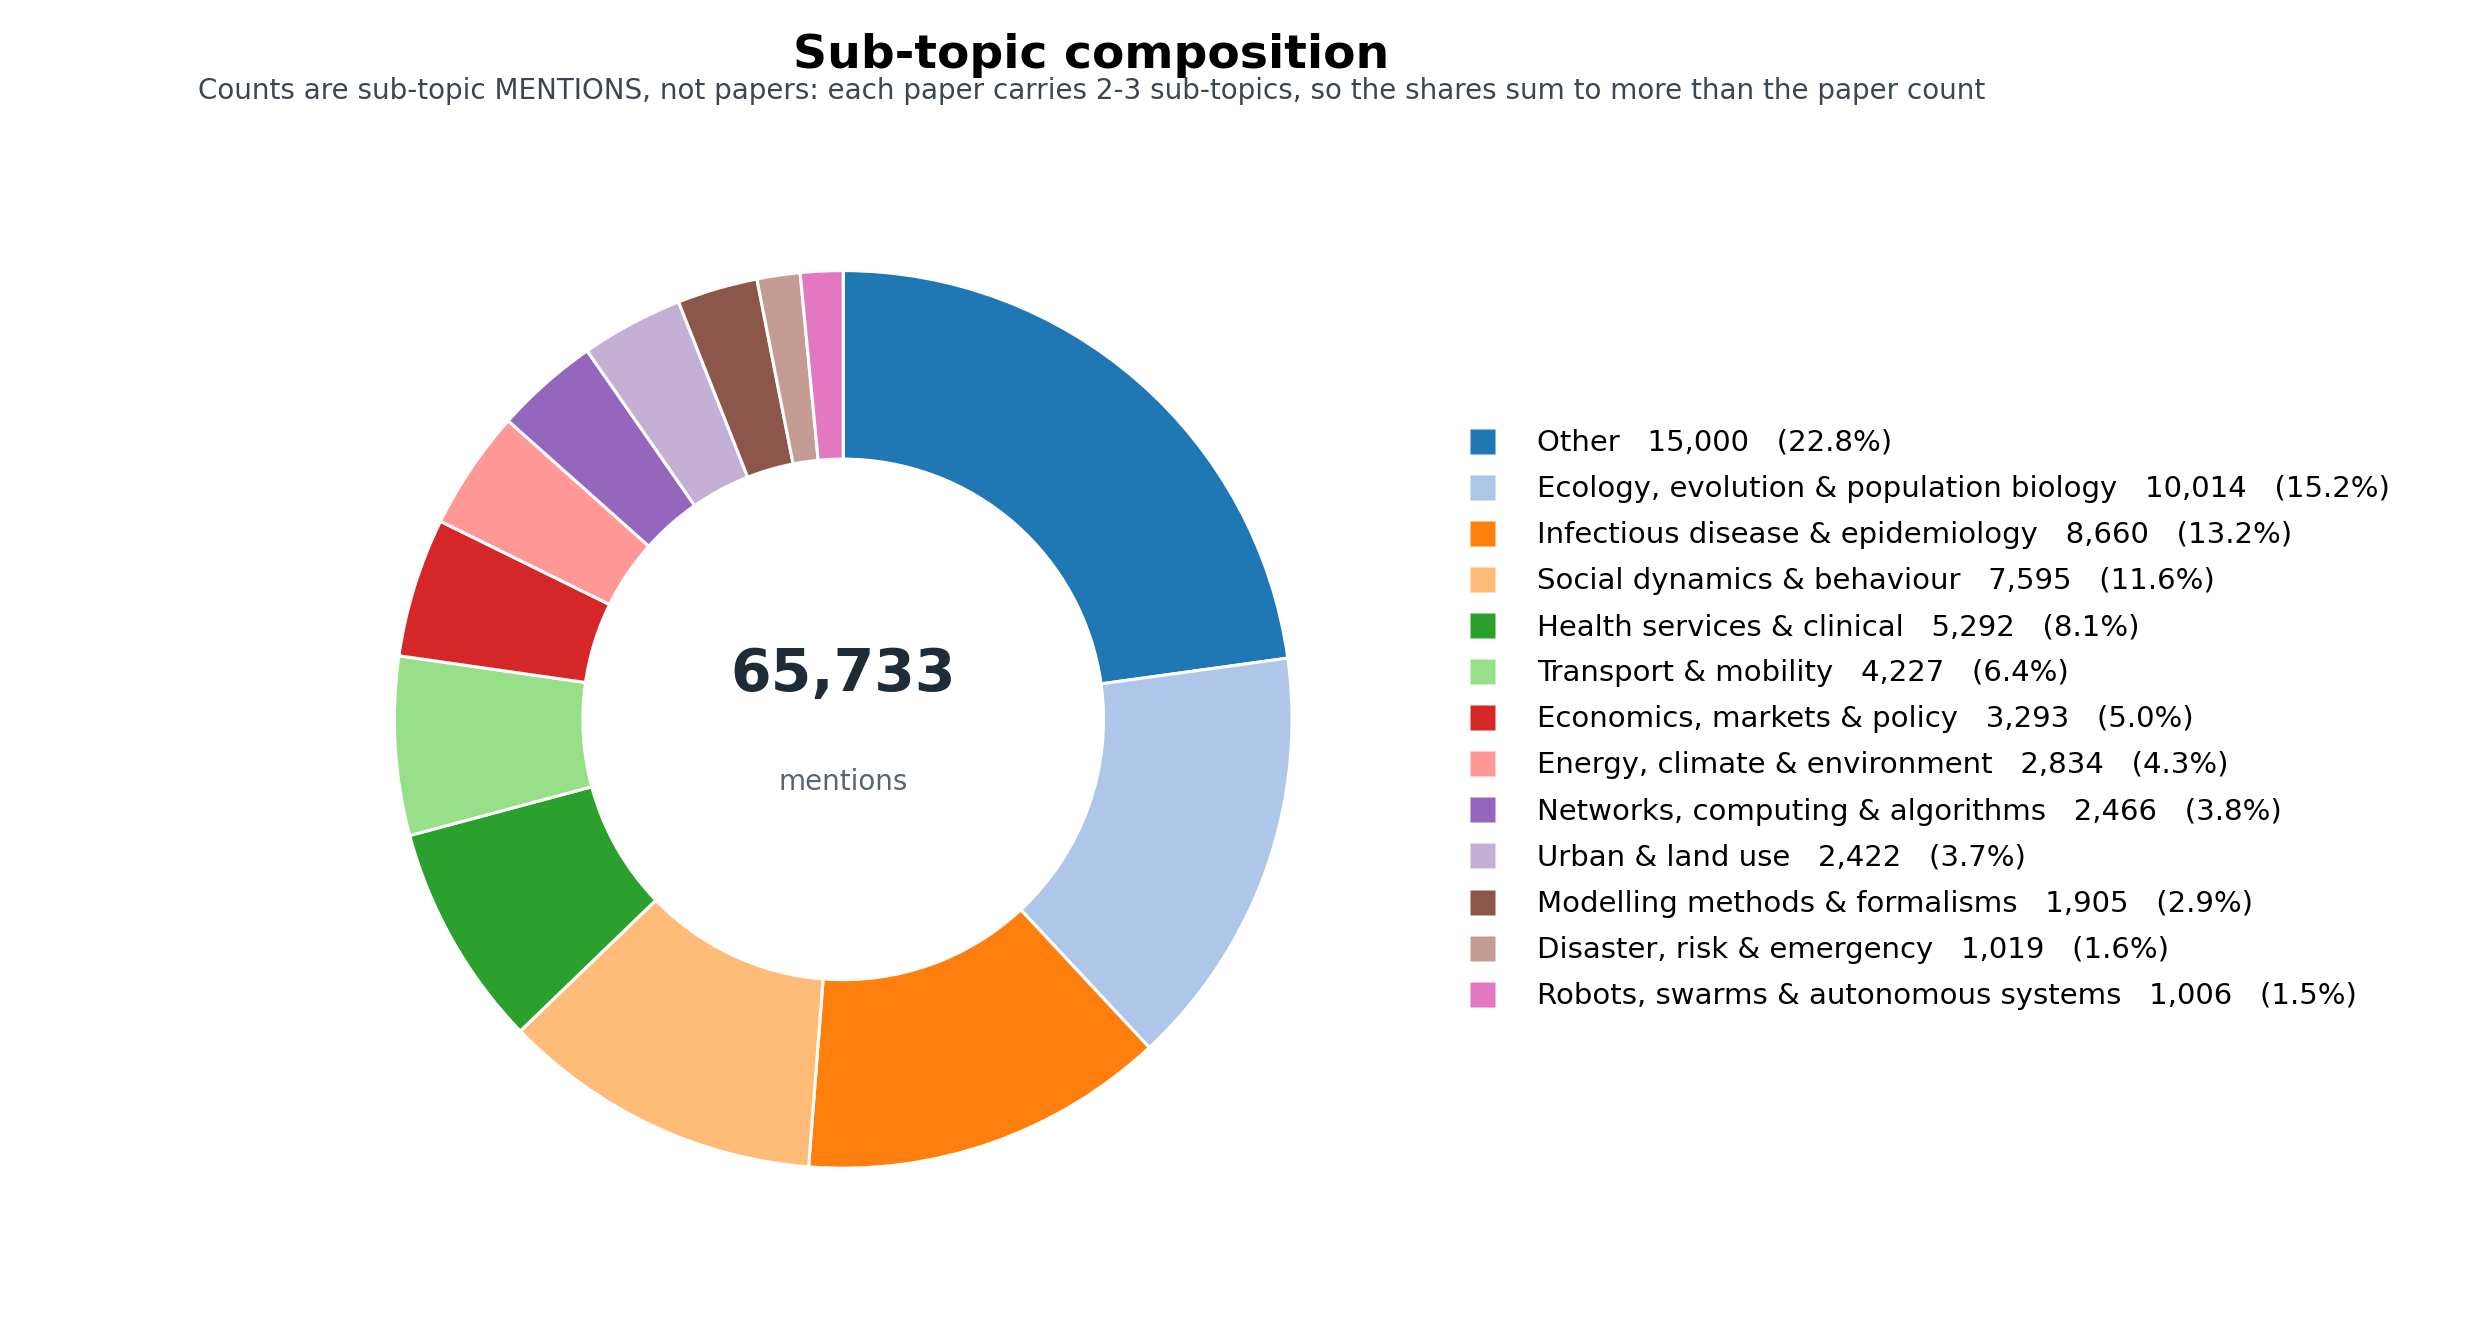
\includegraphics[width=0.96\textwidth,height=0.78\textheight,keepaspectratio]{figures/figure_05.png}
\setcounter{figure}{4}
\caption{Subtheme composition of the corpus.}
\label{fig:figure5}
\end{figure}

Subthemes reveal more detail within the broad domains (Figure 5). Ecology, evolution, and population biology account for 10,014 mentions (15.2\%), followed by infectious disease and epidemiology (8,660; 13.2\%) and social dynamics and behaviour (7,595; 11.6\%). Health services and clinical research (8.1\%) and transport and mobility (6.4\%) are also prominent. These are subtheme mentions, not unique papers: each paper can receive two or three labels. The 65,733 total mentions therefore exceed the corpus size, and percentages represent shares of assigned mentions. “Other” combines less frequent subthemes rather than denoting one substantive topic.

\begin{figure}[htbp]
\centering
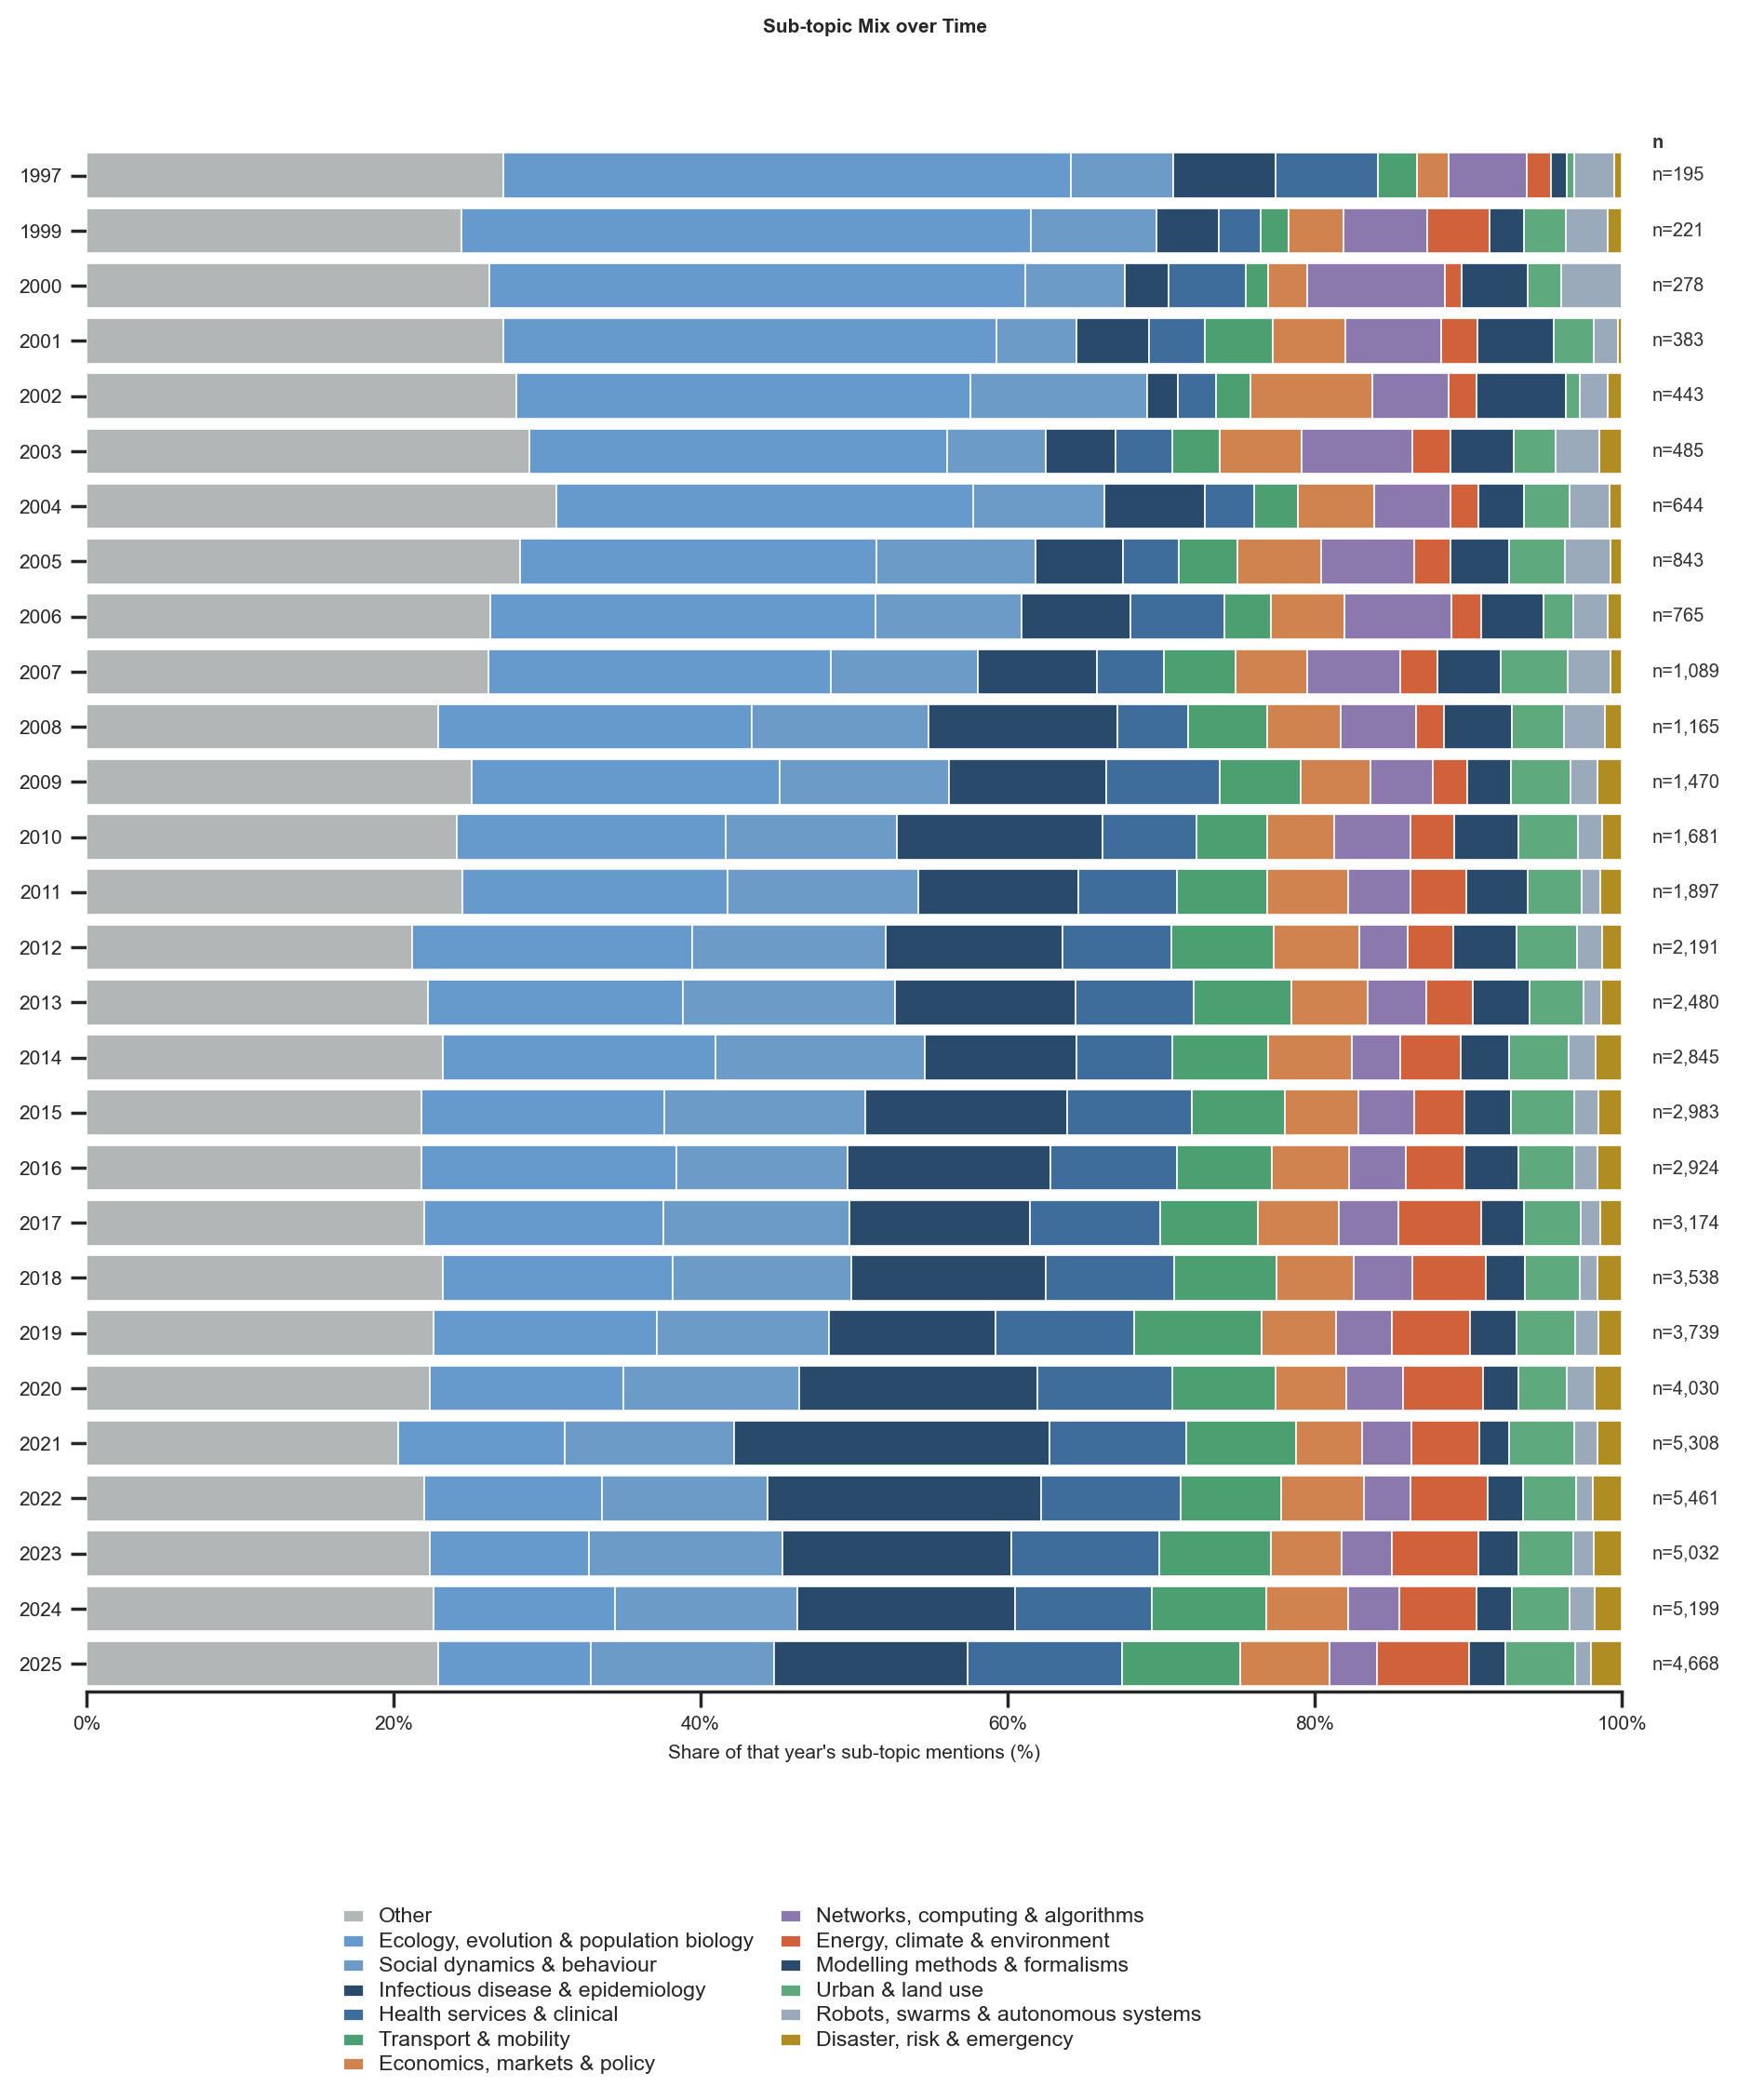
\includegraphics[width=0.96\textwidth,height=0.78\textheight,keepaspectratio]{figures/figure_06.png}
\setcounter{figure}{5}
\caption{Annual evolution of subtheme composition, 1997–2025.}
\label{fig:figure6}
\end{figure}

The annual subtheme series traces this diversification over time. Ecology, evolution, and population biology make up a smaller share of recent annual mentions, while infectious disease and epidemiology and social and behavioural topics account for larger shares. Energy, urban systems, networks, and modeling methods remain smaller but visible parts of the mix. Because the figure reports each year’s share of subtheme mentions, it describes changes in relative emphasis, not absolute publication counts.

Topic co-occurrence offers another view of the corpus’s breadth. Epidemiology/public health co-occurs with health-care systems in 4,476 papers; ecology/environment with policy and disaster response in 2,585; and urban/land-use planning with transport in 1,939 and energy systems in 1,075. These pairings show that many papers are indexed across intersecting application areas rather than isolated topics. Co-occurrence does not, by itself, establish that the topics are integrated within the same model or that one domain influences another.

\begin{figure}[htbp]
\centering
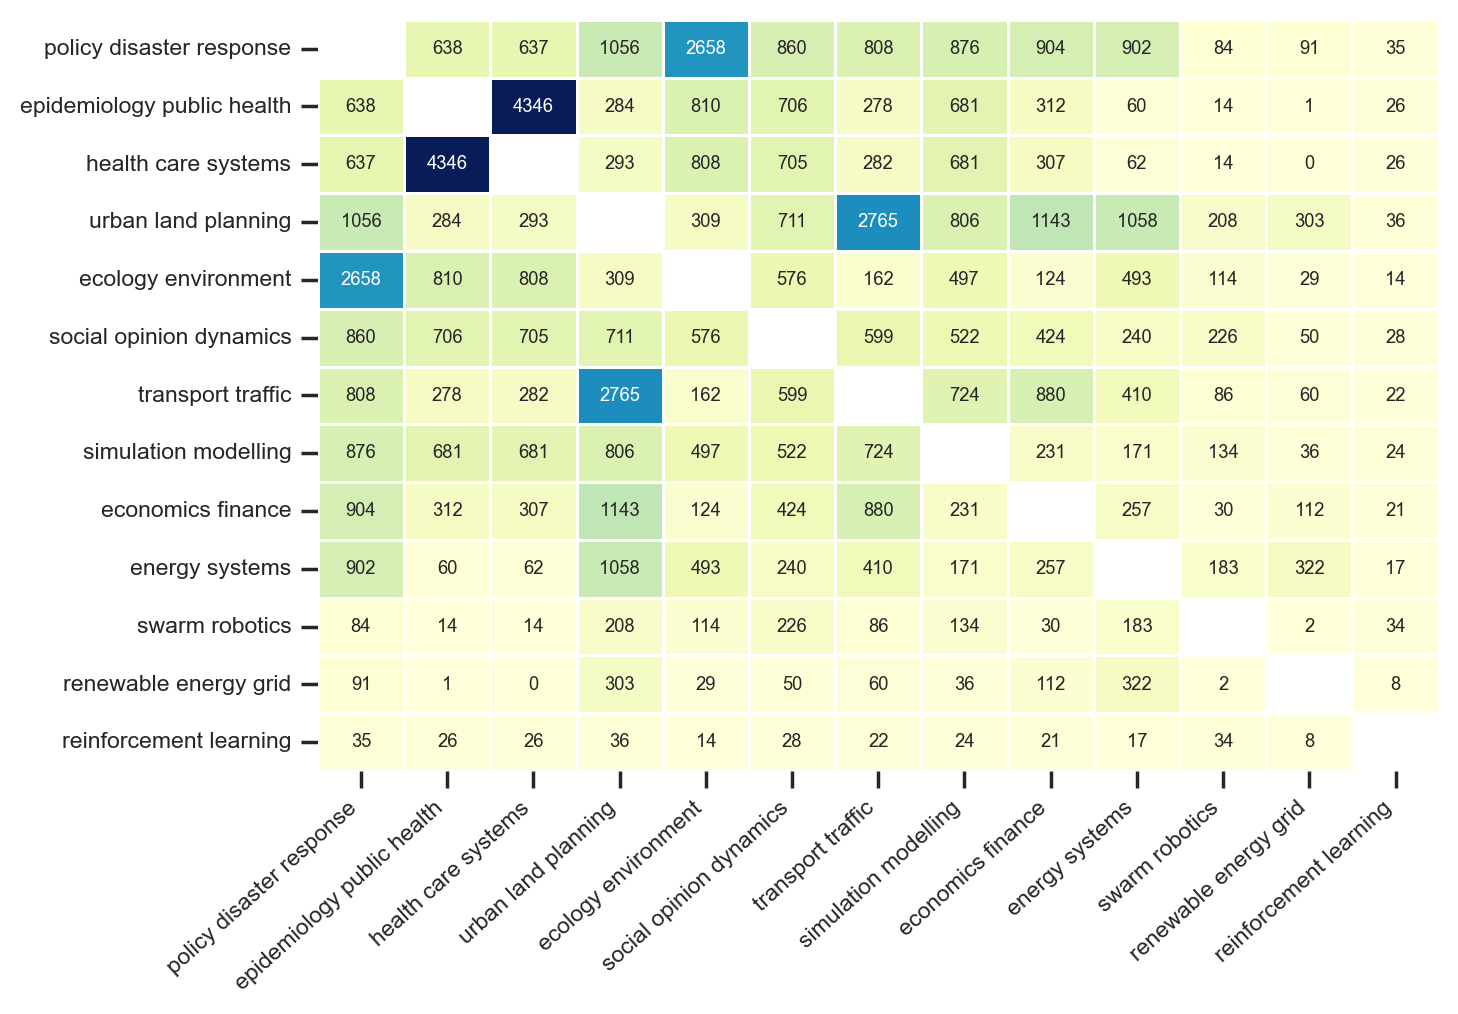
\includegraphics[width=0.96\textwidth,height=0.78\textheight,keepaspectratio]{figures/figure_07.png}
\setcounter{figure}{7}
\caption{Cross-domain co-occurrence intensity.}
\label{fig:figure8}
\end{figure}

This co-occurrence structure reflects ABM’s transferability across disciplinary settings. Its core concepts—heterogeneous agents, local interaction, adaptation, and emergence—can be used to study many kinds of complex systems. The observed links among health, urban systems, transport, environmental processes, and social dynamics therefore suggest that an increasing share of the literature addresses coupled problems. Some models may represent interactions among people, institutions, infrastructure, and the environment, allowing researchers to examine feedback and unintended consequences that aggregate approaches can obscure. The co-occurrence results indicate topical overlap, however, and should not be taken as direct evidence that every paper models these mechanisms jointly.

\subsection{The changing object of simulation}

Humans and households account for 41.20\% of modeled-entity classifications, while patients and other biological entities account for 22.34\%. Decade-based logistic models show a strong increase in human/household representation (OR = 1.483 per decade, q = 1.3 × 10−57) and declines in generalized network nodes, software/computational agents, patients/biological entities, and swarm robots. This shift does not imply that computational or biological models are disappearing. Rather, it signals a growing emphasis on coupled human–environment and human–technology systems, where decisions and interaction networks are themselves part of the causal explanation.

\begin{figure}[htbp]
\centering
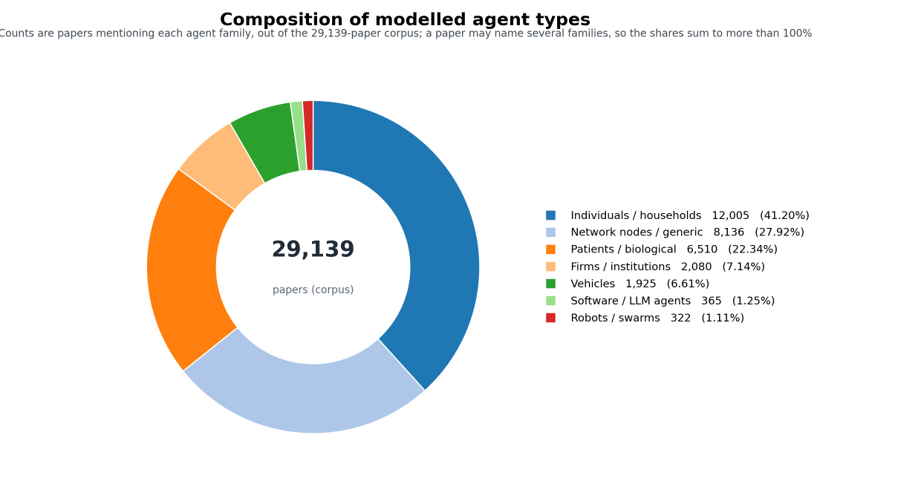
\includegraphics[width=0.96\textwidth,height=0.78\textheight,keepaspectratio]{figures/figure_08.png}
\setcounter{figure}{8}
\caption{Overall composition of modeled agent types.}
\label{fig:figure9}
\end{figure}

\begin{figure}[htbp]
\centering
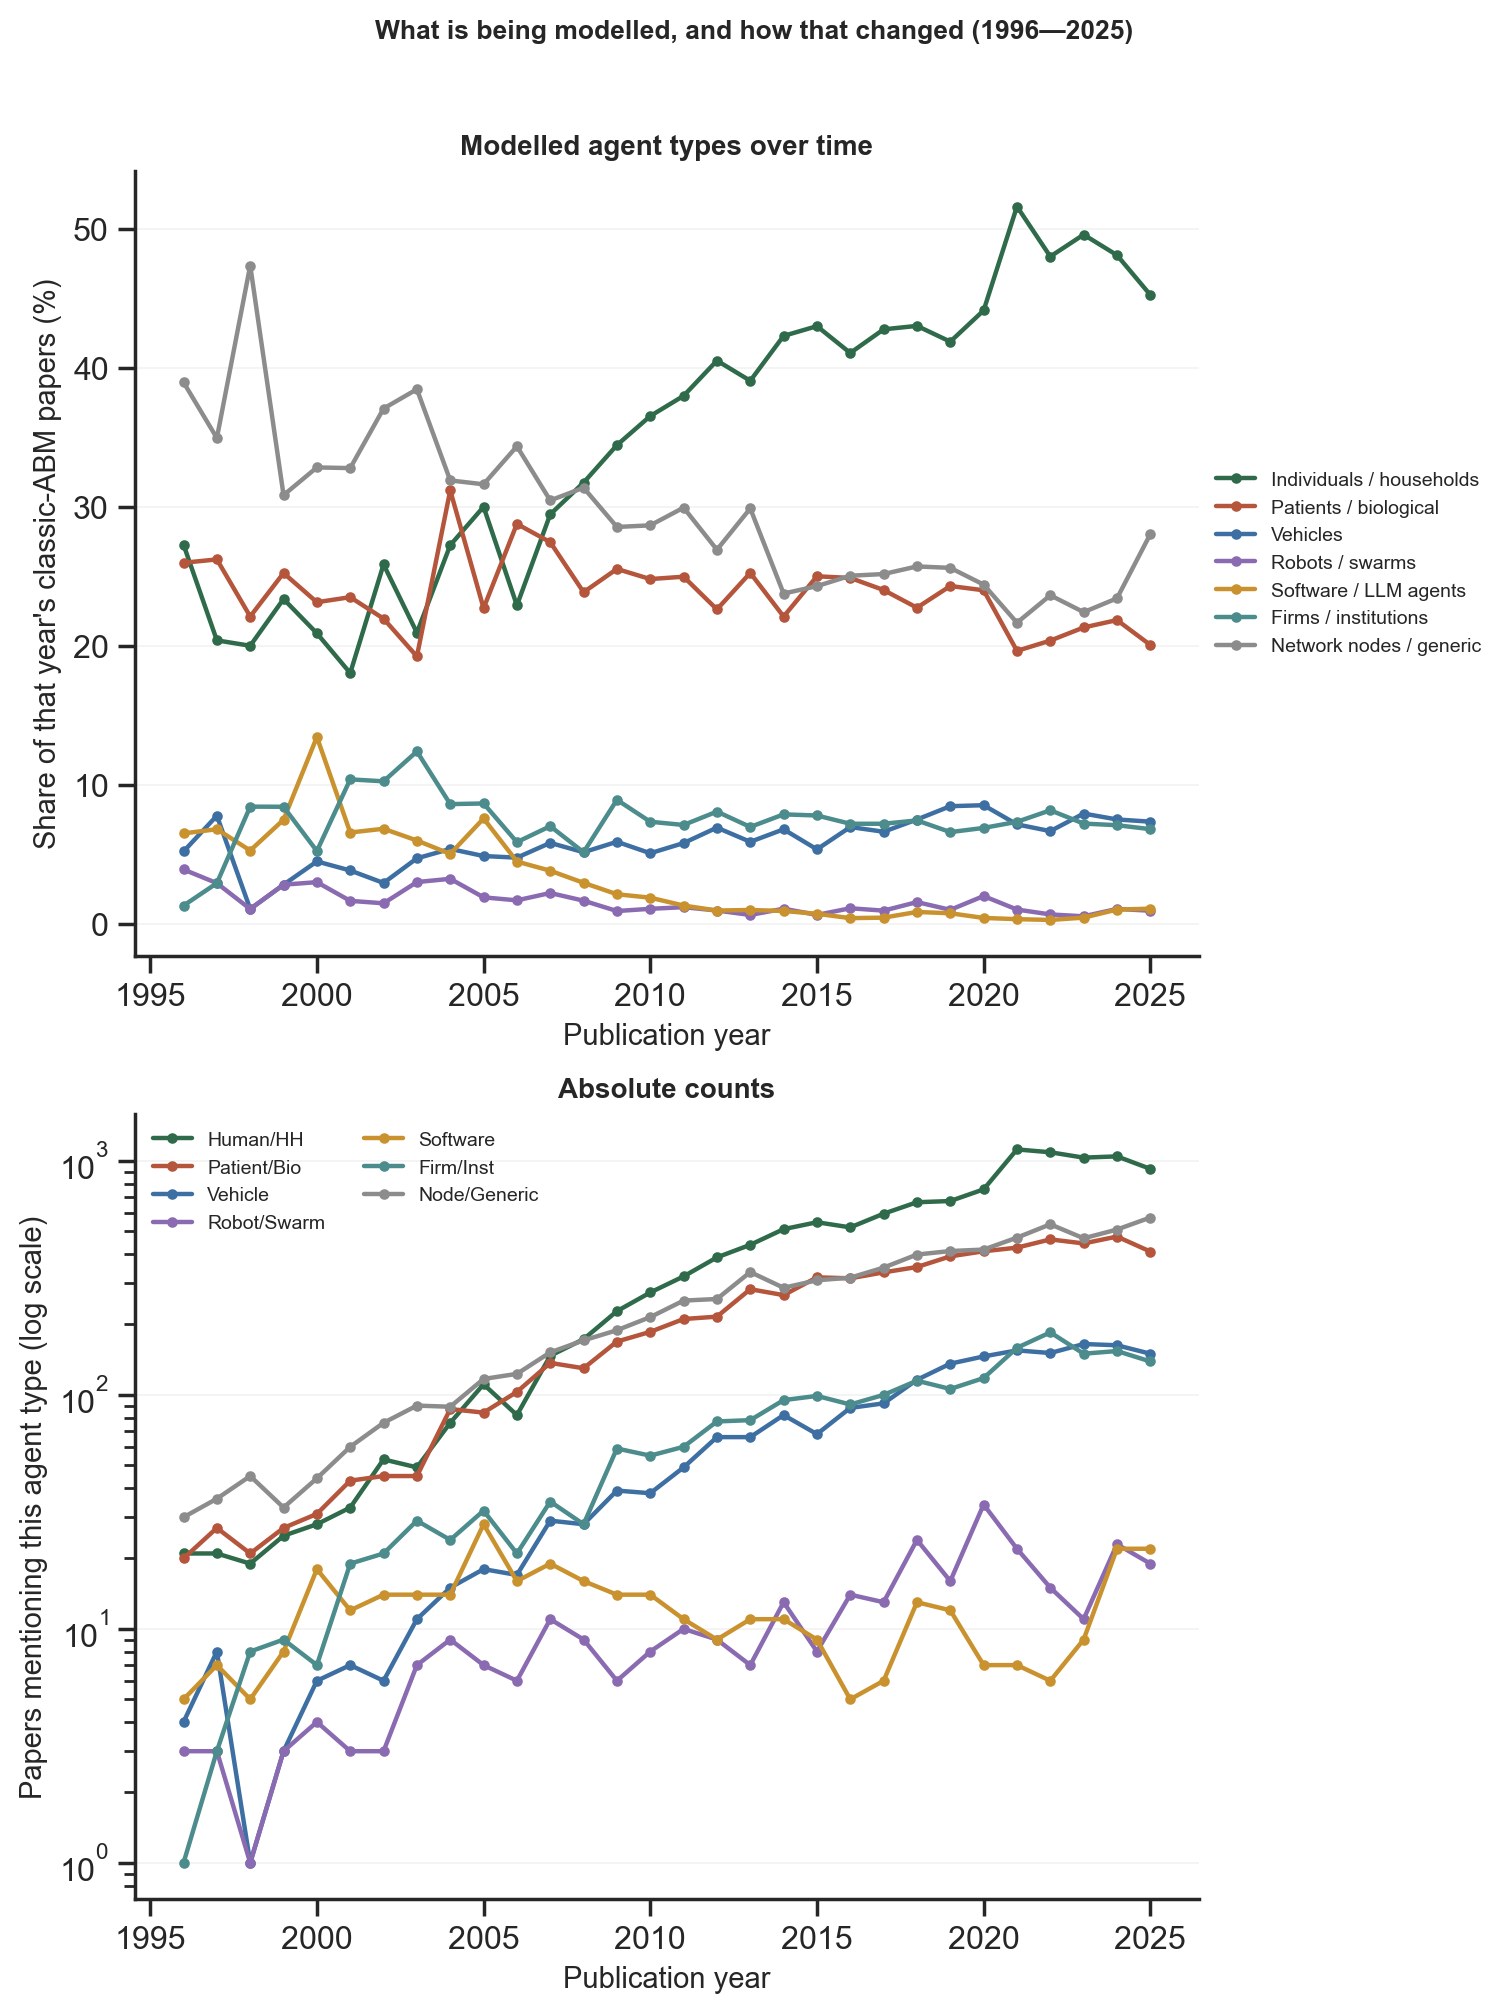
\includegraphics[width=0.96\textwidth,height=0.78\textheight,keepaspectratio]{figures/figure_09.png}
\setcounter{figure}{9}
\caption{Annual trends in modeled agent types, 1996–2025.}
\label{fig:figure10}
\end{figure}

The shift toward human-centered applications sharpens a methodological tension: richer behavioral representations also increase the burden of validation. The ODD protocol and its updates make model structure, design concepts, and implementation details inspectable. As behavioral assumptions become more elaborate, transparent reporting becomes more important, not less. \footnote{Grimm, V., Berger, U., Bastiansen, F., Eliassen, S., Ginot, V., Giske, J., et al. (2006). A standard protocol for describing individual-based and agent-based models. Ecological Modelling, 198(1–2), 115–126. https://doi.org/10.1016/j.ecolmodel.2006.05.023; Grimm, V., Berger, U., DeAngelis, D. L., Polhill, J. G., Giske, J., \& Railsback, S. F. (2010). The ODD protocol: A review and first update. Ecological Modelling, 221(23), 2760–2768. https://doi.org/10.1016/j.ecolmodel.2010.08.019}